\documentclass[12pt]{article}

\usepackage{sbc-template}
\usepackage{graphicx,url}
\usepackage[utf8]{inputenc}
\usepackage[brazil]{babel}
\usepackage{helvet}
\usepackage{caption}
\usepackage{booktabs}
\usepackage{multirow}
\usepackage{array}


\usepackage{times}
\usepackage[T1]{fontenc}
\usepackage{url}
\usepackage{booktabs}
\usepackage{multirow}
\usepackage{graphicx}
\pagenumbering{gobble}
\setlength{\parindent}{1.27cm}
\makeatletter
\renewcommand\@biblabel[1]{}
\makeatother

\DeclareCaptionFont{sbcfont}{\sffamily\bfseries\fontsize{10}{12}\selectfont}
\captionsetup{font=sbcfont, aboveskip=6pt, belowskip=6pt}

     
\sloppy

\title{Radiomics applied to skin lesion classification in HFUS images}

\author{Lucas G. Guedes\inst{1}, Isabela R. V. da Silva\inst{2}, Thatiane A. P. Alva\inst{3}, Viviane R. Botelho\inst{4}}


\address{Departamento de Ciências Exatas e Sociais Aplicadas\\
  Universidade Federal de Ciências da Saúde de Porto Alegre\\
  R. Sarmento Leite, 245 -- 90050-170 -- Porto Alegre -- RS -- Brazil
  \email{\{lucas.guedes, isabelarv, thatiane, vivianerb\}@ufcspa.edu.br}
}

\begin{document} 

\maketitle

\begin{abstract}
This study evaluates the performance of classical machine learning classifiers trained with radiomic features extracted from high-frequency ultrasound images to classify cutaneous lesions according to their malignancy. First-order and texture features were extracted from BW and Doppler images and used to train 22 classifiers, complemented with XGBoost. The best models, both Medium Gaussian SVM, achieved an AUC of 0.96 (BW) and 0.88 (Doppler) on the held-out test set, matching or exceeding a single-modality CNN reported in the literature for the same task. The results indicate that radiomic features alone are sufficient to match the performance of dedicated CNNs.
\end{abstract}


\section{Introduction}

Skin cancer is the most frequently diagnosed neoplasm in the world and also most complex in humans \cite{Juan2023, Zhu2024}. When detected in early stages, the overall survival rate can reach $99\%$, but this effectiveness decrease as the disease progress \cite{Goyal2020}. To make this possible, dermatologists evaluate lesions through different analysis methods as dermatoscopy, confocal microscopy and other images techniques; however, this images are limited in terms of depth of lesion \cite{Xiao2025, Zhu2024}. High-frequency ultrasound helps overcome this limitation by providing high-resolution images from the epidermis to deep fascia, showing potential for differentiating benign and malignant skin lesions \cite{daSilva2026, Czajkowska2021-1}. However, their interpretation remains subjective and dependent on specialist experience, which can lead to diagnostic errors and delays in
reaching a conclusion \cite{Qin2025}

Given this scenario, Machine Learning (ML) and Deep Learning (DL) techniques have emerged as promising tools to assist medical image diagnosis \cite{daSilva2026}. Algorithms based on convolutional neural networks have been widely applied to various medical images modalities, demonstrating performance comparable to human specialists in classification and detection tasks \cite{LaverdeSaad2021}. In HFUS context, LaverdeSaad et al. (2021) explored a single-modality approach, training a pretrained CNN (EfficientNet B4) on color Doppler images, reporting an accuracy of $77.1\%$ on an external test set \cite{LaverdeSaad2021}. Despite these promising results, deep learning models present a relevant limitation for clinical application: their predictions are often difficult to interpret, since the feature extraction process occurs implicitly within the neural network \cite{Qin2025}. Furthmore, effictive neural network training requires a hing computational and data cost \cite{LaverdeSaad2021}. 

In this context, radiomics emerge as a extraction process of a large number of features related to morphological and textural information from medical images, making quantitative information about lesions accessible that is not perceptible through direct visual assessment \cite{Lambin2017}. These extracted characteristics, which include intensity, shape, texture, and wavelet transform values, capture characteristics of the lesion's phenotype that are distinct from or complementary to information obtained by other methods \cite{Lambin2017}.

Despite growing interest in radiomics for medical imaging, few studies have applied it to ultrasound-based skin tumor classification, with most relying on DL instead \cite{Surkov2024, Bibi2026, Czajkowska2021-2}. Given this gap, the present work aims to evaluate the performance of several classical machine learning classifiers trained with
radiomic features extracted from HFUS images to assess the malignancy of
cutaneous lesions, comparing the results obtained with those reported by laverde-saad et al. (2026)

\section{Materials and Methods}
\subsection{Dataset and Feature Extraction}
The dataset used was produced by Alfageme et al. \cite{Alfageme2022}, comprising 240 $\times$ 240 px PNG HFUS images (BW and Doppler modes) of cutaneous lesions, labeled as benign (65.7\%) or malignant (34.3\%). Images were stratified into 70\% train / 30\% test subsets to preserve class proportions. Prior to extraction, dataset inconsistencies documented by Silva et al. (2026)

Radiomic features were extracted using PyRadiomics, yielding 465 first-order and texture features per image, calculated on the original image and on the four sub-bands of the 2D wavelet decomposition (LL, LH, HL, HH), which capture spatially localized frequency content otherwise suppressed in the original image. Two feature datasets were created: BW, Doppler.

\subsection{Experimental Design and Evaluation}
% Given the high number of features, SelectKBest (scikit-learn) was used to rank feature relevance on the training set with two criteria: the ANOVA F-score (inter-/intra-class variance ratio) and Mutual Information (non-linear feature-target dependence), both computed on the training set only to avoid data leakage.

All extracted features were standardized (StandardScaler) and used in their entirety to train each of two datasets (BW, Doppler) on same 22 classifiers used in Faita et al. (2021) and complemented with XGBoost \cite{Faita2022}. Performance was estimated via stratified 5-fold cross-validation on the training set. The classifier with the highest mean cross-validation AUC per dataset was retrained on the full training set and evaluated once on the held-out test set, using both a 0.5 threshold and the Youden-index threshold; AUC, accuracy, sensitivity, specificity, and F1-score were computed for each.

\section{Results and Discussion}

Table \ref{tab:resultados-youden} presents the held-out test set performance, at youden threshold, of the classifier with the highest mean AUC in cross-validation. Compared to the single-modality EfficientNet B4 trained on color Doppler images by Laverde-Saad et al. (2021), which achieved an accuracy of 77.1\%, sensitivity of 71\%, specificity of 80\%, and AUC of 0.78 on an external test set \cite{LaverdeSaad2021}, our Doppler-based Medium Gaussian SVM achieved an accuracy of 85\%, sensitivity of 0.57, specificity of 1.00, and AUC of 0.88, indicating a trade-off toward fewer false positives at the cost of more false negatives. The BW-based classifier, in turn, achieved the highest overall discrimination among the three, with an AUC of 0.96, accuracy of 85\%, sensitivity of 71\%, and specificity of 92\%.

\begin{table}[ht]
    \centering
        \caption{Performance of the best classifiers per dataset in youden threshold (on the test data) - Tracks A and B}
        \label{tab:resultados-youden}
        \resizebox{0.8\textwidth}{!}{%
        \begin{tabular}{clcccccc}
        \toprule
        \textbf{Track} & \textbf{Dataset} & \textbf{Model} & \textbf{Sens.} & \textbf{Spec.} & \textbf{F1} & \textbf{Acc.} & \textbf{AUC} \\
        \midrule
        \multirow{3}{*}{B} 
            & BW         & Medium Gaussian SVM    & 0.71 & 0.92 & 0.77 & 0.85 & 0.96 \\ 
            & Doppler    & Medium Gaussian SVM    & 0.57 & 1.00 & 0.73 & 0.85 & 0.88 \\
        \bottomrule
    \end{tabular}}
\end{table}

Taken together, these results indicates that radiomic features extracted from HFUS images can support accurate classification of cutaneous lesions, with performance comparable to or exceeding that of CNN-based, such as the EfficientNet B4 architecture used by Laverde-Saad et al. (2021). The models in this study as trained in approximately 51ms on a conventional CPU (Intel Core i5-7267U, 8GBs RAM), without any GPU usage.

Figure \ref{fig:predicted-scores} shows the predicted malignancy probability per test sample (BW and Doppler, Medium Gaussian SVM): benign samples cluster near 0.05--0.20 and malignant samples near 0.70--0.95, with few samples falling between the Youden and 0.5 thresholds.

This pattern reinforces the  discriminative confidence suggested by qunatitative results: defining the region between the Youden and 0.5 thresholds as a zone of uncertainty, this zone is sparsly populated for both datasets, indicating strong discriminative confidence. 

\begin{figure}[h]
    \centering
    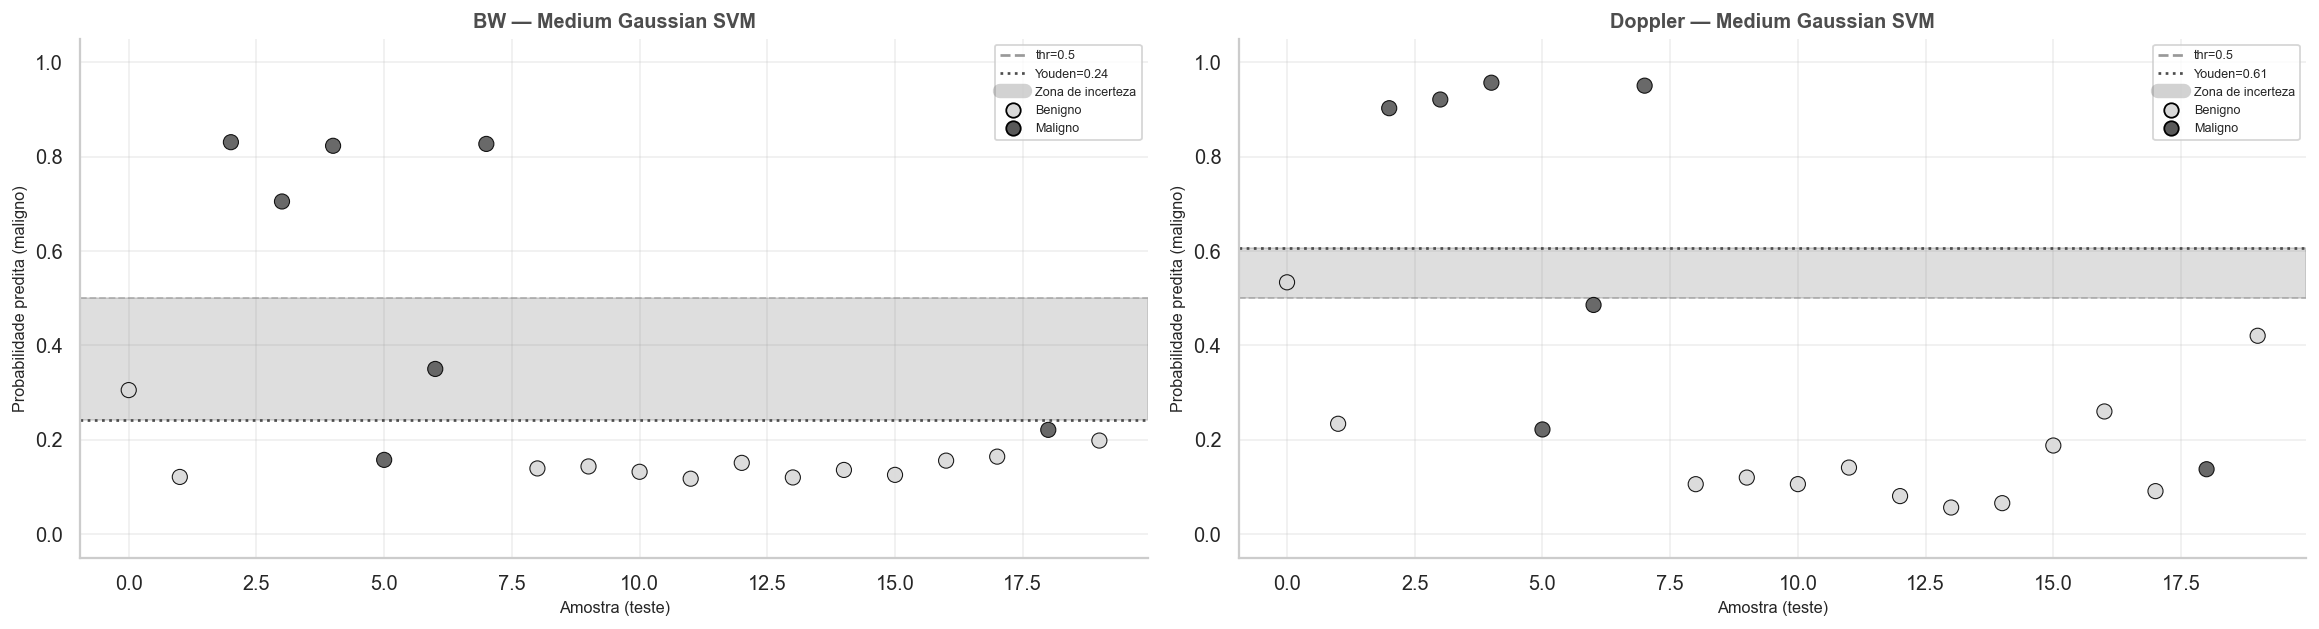
\includegraphics[width=\textwidth]{images/Scatter-grey.png}
    \caption{Predicted probability of malignancy on the test set, per sample, for BW and Doppler (Medium Gaussian SVM). Dashed line: 0.5 threshold; dotted line: Youden threshold.}
    \label{fig:predicted-scores}
\end{figure}

A limitation of this study is the small test set (n=20: 13 malignant, 7 benign), which limits the stability of point estimates; results should therefore be regarded as preliminary evidence requiring confirmation on larger datasets.

This work shows that classical machine learning classifiers trained on radiomic features extracted from HFUS images can match or exceed CNN-based approaches for benign/malignant skin lesion classification. Future work should validate these findings on larger, multi-center datasets.

\begin{thebibliography}{99}
\setlength{\leftmargin}{0.5cm}
\setlength{\itemindent}{-0.5cm}
\setlength{\itemsep}{6pt}
\setlength{\parsep}{0pt}
\bibitem[Alfageme 2022]{Alfageme2022} Alfageme, F. (2022). Dermatologic ultrasound images for classification. \url{https://www.kaggle.com/datasets/alfageme/dermatologic-ultrasound-images}.

\bibitem[Bibi et al. 2026]{Bibi2026} Bibi, F., Abbas, Q. and Naqi, S. M. (2026) dual-stream deep learning model for early detection and classification of non-dermoscopic skin lesions via focal modulation and local feature integration. \textit{IEEE Access}, 14:41998--42014.

\bibitem[Czajkowska et al. 2021a]{Czajkowska2021-1} Czajkowska, J., Badura, P., Korzekwa, S., P{\l}atkowska-Szczerek, A. and S{\l}owi{\'n}ska, M. (2021). Deep learning-based high-frequency ultrasound skin image classification with multicriteria model evaluation. \textit{Sensors}, 21(17):5846.

\bibitem[Czajkowska et al. 2021b]{Czajkowska2021-2} Czajkowska, J., Badura, P., Korzekwa, S. and P{\l}atkowska-Szczerek, A. (2021). Deep learning approach to skin layers segmentation in inflammatory dermatoses. \textit{Ultrasonics}, 114:106412.

\bibitem[Faita et al. 2022]{Faita2022} Faita, F., Oranges, T., Di Lascio, N., Ciompi, F., Vitali, S., Aringhieri, G., Janowska, A., Romanelli, M. and Dini, V. (2022). Ultra-high-frequency ultrasound and machine learning approaches for the differential diagnosis of melanocytic lesions. \textit{Experimental Dermatology}, 31(1):94--98.

\bibitem[Goyal et al. 2020]{Goyal2020} Goyal, M., Knackstedt, T., Yan, S. and Hassanpour, S. (2020). Artificial intelligence-based image classification methods for diagnosis of skin cancer: challenges and opportunities. \textit{Computers in Biology and Medicine}, 127:104065.

\bibitem[Juan et al. 2023]{Juan2023} Juan, C. K., Su, Y. H., Wu, C. Y., et al. (2023). Deep convolutional neural network with fusion strategy for skin cancer recognition: model development and validation. \textit{Scientific Reports}, 13(1):17087.

\bibitem[Lambin et al. 2017]{Lambin2017} Lambin, P., Leijenaar, R. T., Deist, T. M., et al. (2017). Radiomics: the bridge between medical imaging and personalized medicine. \textit{Nature Reviews Clinical Oncology}, 14(12):749--762.

\bibitem[Laverde-Saad et al. 2021]{LaverdeSaad2021} Laverde-Saad, A., Jfri, A., Garc\'ia, R., et al. (2021). Discriminative deep learning based benignity/malignancy diagnosis of dermatologic ultrasound skin lesions with pretrained artificial intelligence architecture. \textit{Skin Research and Technology}, 28(1):35--39.

\bibitem[Qin et al. 2025]{Qin2025} Qin, Y., Zhang, Z., Qu, X., Liu, W., Yan, Y. and Huang, Y. (2025). A machine learning model based on high-frequency ultrasound for differentiating benign and malignant skin tumors. \textit{Medical Ultrasonography}, 27(3):284--293.

\bibitem[Silva et al. 2026]{daSilva2026} Silva, I. R. V. da, Jardim, A. G., Fa\'es, G. R. da S., Alva, T. A. P., Becker, C. D. L. and Botelho, V. R. (2026). Deep learning-based skin lesion classification: a CNN approach on high-frequency ultrasound imaging. \textit{Journal of Ultrasound in Medicine}, 45(5):925--936.

\bibitem[Surkov et al. 2024]{Surkov2024} Surkov, Y. I., Serebryakova, I. A., Kuzinova, Y. K., et al. (2024). Multimodal method for differentiating various clinical forms of basal cell carcinoma and benign neoplasms in vivo. \textit{Diagnostics}, 14(2):202.

\bibitem[Xiao et al. 2025]{Xiao2025} Xiao, C., Zhu, A., Xia, C., et al. (2025). Attention-guided learning with feature reconstruction for skin lesion diagnosis using clinical and ultrasound images. \textit{IEEE Transactions on Medical Imaging}, 44(1):543--555.

\bibitem[Zhu et al. 2024]{Zhu2024} Zhu, A. Q., Wang, Q., Shi, Y. L., et al. (2024). A deep learning fusion network trained with clinical and high-frequency ultrasound images in the multi-classification of skin diseases in comparison with dermatologists: a prospective and multicenter study. \textit{eClinicalMedicine}, 67:102391.
\end{thebibliography}


\end{document}
